
\section{Genom Annotation (Einführung)} \index{Genom-Annotation}
\begin{mybox}[title=Definition Genom-Annotation]
Identifizierung der Lage aller Gene und Kodierregionen in einem Genom + Bestimmung der Funktion der Gene
\end{mybox}
\subsection{Überblick}
\begin{figure}[H]
    \centering
    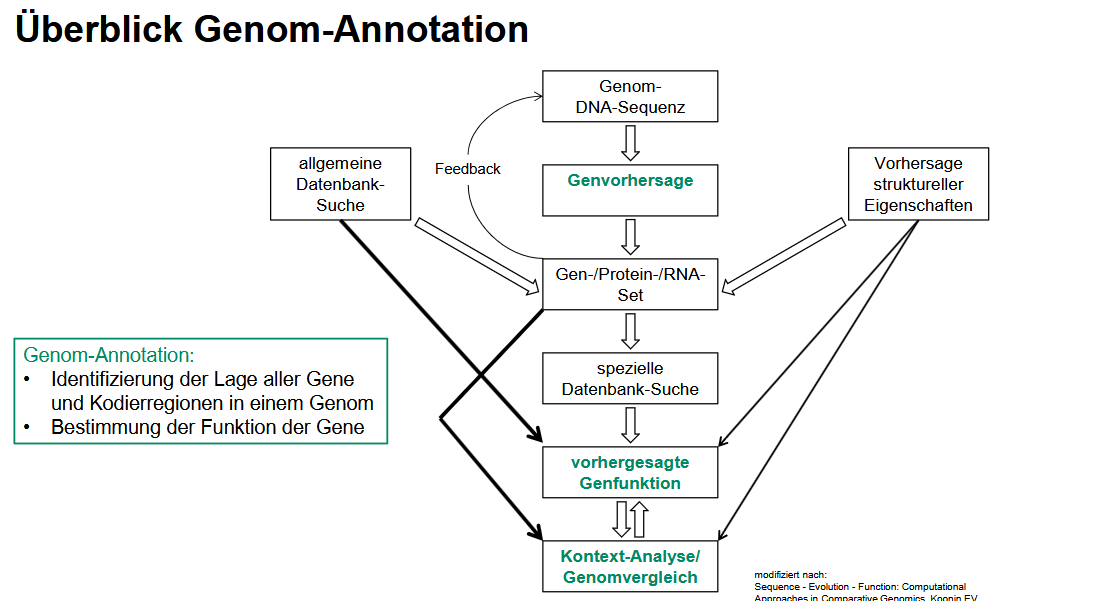
\includegraphics[width=1.2\linewidth]{images/genom annotation.PNG}
    \caption{Diagramm zum Ablauf von Genom Annotationen}
    \label{fig:enter-label} 
\end{figure}

\subsection{GC Gehalt und GC Skew} \index{GC Skew}
Der GC Gehalt ist eine prozentuelle Anzahl von den Basen G und C in der DNA Sequenz. 
Solches ist: 
\begin{itemize}
    \item taxonomisches Merkmal von Mikroorganismen
    \item Ein Hinweis auf Ursprung / Herkunft des Replikons oder Region.
    \item in Kodierregionen oft erhöht.
\end{itemize} 
Der GC Gehalt wird wiefolgt berechnet: 
\[
\%GC\text{-Gehalt} = \frac{\#G + \#C}{\#A + \#T + \#G + \#C} \times 100 = \frac{\#G + \#C}{\#Alle \ Basen} \times 100
\]\\
\gls{GC-Skew} ist ein Maß für die Asymmetrie der Verteilung von Guanin (G) und Cytosin (C) in einer DNA-Sequenz. Das bedeutet, dass es prüft, ob Guanin und Cytosin in einer bestimmten Region der DNA oder RNA über- oder unterexprimiert sind.
Die Formel hierfür ist wiefolgt:
\[
GC_{window} = \frac{(\#G_{window} - \#C_{window})}{(\#G_{window} + \#C_{window})}
\]\\
Wobei w eine Sequenzfenster darstellt.\\
Das anwenden beider Metriken kann zum finden eines Replikationsursprung benutzt werden.  

\subsection{Lokalisation von Genen} 
\paragraph{Wie kann man Gene lokalisieren?} Durch Computeranalyse (Das Auffinden von Sequenzmerkmalen, die mit Genen assoziiert) oder experimentelle Analyse (z.B. Analyse und Charakterisierung von Mutanten).
\paragraph{Wichtig zu wissen ist} Gene enthalten offene Leseraster \index{Leseraster}
(\gls{orf}) und alles zwischen Start und Stopp ist das \gls{orf}. Dabei ist die Verteilung von Stopcodons ist nicht zufällig. 
\begin{itemize}
    \item \gls{orf} Startcodons sind: ATG, GTG, TTG \index{Startcodon}
\item \gls{orf} Stoppcodons sind: TAA, TAG, TGA \index{Stoppcodon}
\end{itemize}
\begin{mybox}[title=Wie gibt es für eine Sequenz verschiedene Leseraster? 
Wie viele Leseraster kann es geben?]
Da ein Codon 3 Basen umfasst, kann man an Position 1, 2 oder 3 beginnen. Also gibt es drei verschiedene Einteilungen desselben Strangs in Tripletts. Zusätzlich kann der komplementäre Gegenstrang in 3'-→5'-Richtung gelesen werden, was ebenfalls 3 Leseraster ergibt. Also insgesamt 6. 
\end{mybox}
Man kann mit Computerprogrammen nach Genen durch \gls{orf} Start / Stopp scannen (ORF-Scanning). \index{ORF-Scanning}
Ablauf:
\begin{enumerate}
    \item Festlegung von minimaler \gls{orf} länge
    \item Suche nach "Stop"
    \item Anschließend suche nach entferntestem "Start"
\end{enumerate}
Hierbei werden alle sechs Leseraster gescannt.
\paragraph{WICHTIG:} Bakterielle Gene haben meißt keine (oder so gut wie keine) Überlappung!
Außerdem ist bei Eukaryonten die großen intergenischen Bereiche ein Problem, da solche zu Falschvorhersagen führen können!

\begin{mybox}[title=Die \gls{rbs}]
Eine kurze Sequenz (~5–10 bp) im 5'-UTR prokaryotischer mRNAs, typischerweise 5–10 bp stromaufwärts des Startcodons. Die Konsensussequenz lautet AGGAGG (Shine-Dalgarno-Sequenz). Sie ist komplementär zur 3'-Region der 16S rRNA der kleinen Ribosomenuntereinheit. D.h. die Hybridisierung positioniert das Ribosom am Startcodon. Bei der Genomannotation dient die RBS als Hinweis auf den tatsächlichen Translationsstart eines vorhergesagten ORFs. 
\end{mybox}
\begin{mybox}[title=Definition Frameshift]
Eine Mutation, bei der eine Anzahl von Basen eingefügt oder entfernt wird, die kein Vielfaches von 3 ist. Dadurch verschiebt sich das Leseraster ab der Mutationsstelle vollständig und alle nachfolgenden Codons werden anders gelesen.
\end{mybox}

\subsection{Bessere Methoden zur Genvorhersage}
Es gibt extrinsische Methoden und intrinsische Methoden (Ab initio Methoden).  Bei extrinsischen Methoden finden ein Abgleich mit bereits bekannten Genen und Ähnlichkeitsvergleiche (mRNA,Proteine, cDNAs, \glspl{est}) statt. Bei intrinsischen Methoden wird nach Sequenzmustern gesucht, bspw. nach Promotor-Elementen, Spleißstellen, Exon- und Intronlänge oder der Verteilung von Stopcodons. 

Ein Beispiel für eine intrinsische Methode ist die Genvorhersage mit Glimmer (basiert auf Hidden Markov Modell).

\subsection{Datenbanken für extrinsische Abgleiche} \index{Datenbank}
\begin{table}[H]
    \centering
    \begin{tabular}{p{8cm}p{7cm}}
      \textbf{Datenbanktyp}   & \textbf{Merkmale} \\ \\
      \textbf{Nukleinsäure-Sequenz Datenbanken } & täglicher Datenaustausch, identische Rohdaten  \\ \\ \index{Datenbank!Nukleinsäure-Sequenz}
       \textbf{Genome Browser } &  bietet Rahmen für die Organisation der Daten eines
Organismus\\ \\
        \textbf{Protein-Sequenz Datenbanken} &  Protein Information Resource \\ \\ \index{Datenbank!Protein-Sequenz}
       \textbf{ Struktur-Datenbanken} &  experimentell bestimmte Strukturen von Proteinen\\ \\ \index{Datenbank!Struktur-} 
       \textbf{Expressions- und Proteomics-Datenbanken}  &  Messungen von mRNA bzw. Protein levels, beschreiben Transkriptions- bzw. Translationsmuster\\ \\ \index{Datenbank!Proteomics-} \index{Datenbank!Expressions}
        \textbf{Datenbanken für Metabolic Pathway}s & Sammlung individueller Genome, Genprodukte und ihrer Funktion, insbesondere Integration biochemischer und genetischer Information \index{Datenbank!Metabolic Pathway}
    \end{tabular}
    \caption{Datenbanktypen für die Molekularbiologie und ihre Merkmale.}
    \label{tab:my_label}
\end{table}

\begin{table}[H]
    \centering
    \begin{tabular}{l l|l|l}
    \textbf{Name} & & \textbf{Eingabe Seq.} & \textbf{Gesuchte Seq.} \\ \hline
        blastn & - nucleotide blast  & Nukleotid & Nukleotid  \\
        blastp & - protein blast & Protein & Protein \\
        blastx & & Tranlatierte Nukleotid & Protein \\
        tblastn & & Protein & Tranlatierte Nukleotid \\
        tblastx & & Tranlatierte Nukleotid & Tranlatierte Nukleotid 
    \end{tabular}
    \caption{Arten von BLAST-Suchen.}
    \label{tab:my_label}
\end{table}

% Folie 20 vielleicht irgendwann mal noch 

\subsection{Homolog, ortholog und paraloge Gene} \index{Homolog} \index{Paralog} \index{Ortholog}

\begin{figure}[H]
    \centering
    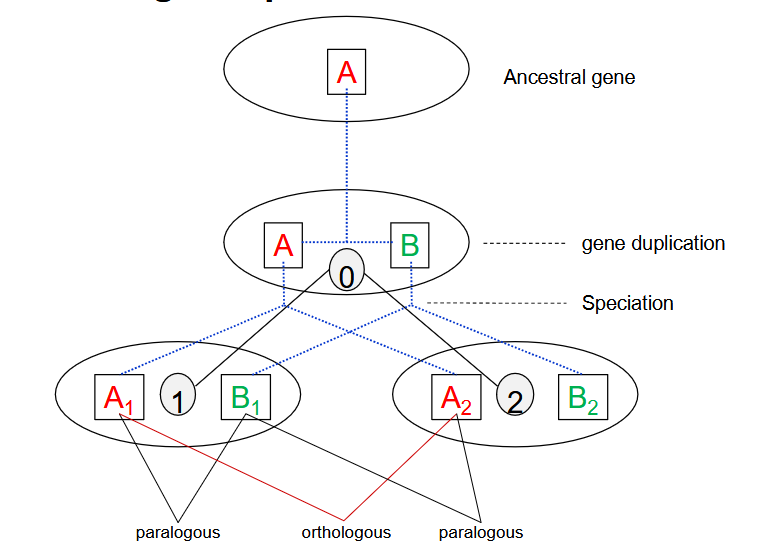
\includegraphics[width=0.7\linewidth]{images/hop.PNG}
    \caption{Beispiel für Ortholog und Paralog}
    \label{fig:enter-label}
\end{figure}
\begin{mechanism}[title=Erklären Sie die Begriffe Ortholog\, Paralog und Homolog]
\begin{itemize}
    \item homolog: Zwei Gene (oder Proteine) sind zueinander homolog, wenn sie von einem gemeinsamen Vorläufer abstammen.
Meist basieren Homologie-Zuweisungen auf Ähnlichkeiten in Sequenz oder Struktur
\item ortholog: homologe Gene, die in verschiedenen Organismen vorkommen und auf einen gemeinsamen Vorfahren
zurückgehen, der vor der Aufspaltung der Art existierte. Orthologe Gene haben in der Regel die gleichen oder sehr ähnliche
Funktionen.
\item paralog: homologe Gene, die durch ein Duplikationsereignis im Genom entstanden sind. Es handelt sich um neue Gene, die
neue (häufig dem Ursprungsgen noch ähnliche) Funktionen kodieren. Paraloge Gene befinden sich häufig im selben Genom
\end{itemize}
\end{mechanism}
\subsection{\gls{cogs} von Proteinen}
\gls{cogs} sind phylogenetische Klassifikation von Proteinen, die in vollständigen Genomen kodiert sind. Jedes Cluster enthält dabei Proteine oder Gruppen von
Paralogen von mindestens drei phylogenetischen Linien. 

\subsection{Eigenschaften von Genen}
\begin{itemize}
    \item Genname \textit{(basierend auf Konfidenz und Kriterien wie nahe verwandten Organismen)}
    \item Genprodukt \textit{(basierend auf Konfidenz und offiziellen Namen)}
    \item Funktion des Genprodukts
    \item \gls{Evidenz}
    \item \gls{ecnummer} \index{E.C Nummer}
\end{itemize}
\section{Komparative Genomik} \index{omparative Genomik}
\paragraph{Komparative Genomik} ist die Analyse und der Vergleich von Genomen unterschiedlicher Spezies.
\begin{itemize}
    \item Einblicke in genomische Struktur unterschiedlicher Spezies
    \item Besseres Verständnis zur Evolution
    \item Funktion und nicht kodierende Regionen bestimmen
    \item Verbesserung bestehender Gen-Annotationen erreichen.
\end{itemize}
\paragraph{Vergleichbare Eigenschaften} von Genomen sind:
\begin{itemize}
    \item Sequenz-Ähnlichkeit
    \item Gen-Lokalisation
    \item Länge und Anzahl kodierender Regionen
    \item Menge/Umfang nichtkodierender DNA
    \item konservierte Regionen
\end{itemize}
Aufgrund zunehmender Verfügbarkeit vollständig sequenzierter Genome nicht mehr auf Abschnitte beschränkt, sondern auf alle Gene und deren Anordnung anwendbar.

\paragraph{Vergleich von Genomen unterschiedlicher phylogenetischer Distanzen} eignen sich, um unterschiedliche Fragestellungen zu bearbeiten. 
\begin{itemize}
    \item Große Gruppen von (weit entfernten) Organismen: Was sind die Basisproteine aller Organismen dieser Gruppe? 
    \item Organismen mit moderatem Abstand: Welche Sequenzen sind funktional? 
    \item Eng verwandte Organismen: Welche Sequenzen führen zu den speziellen Eigenschaften des Organismus?
\end{itemize}


\paragraph{Die Taxonomie} \index{Taxonomie} ist eine Klassifikations Prinzip der Biologie.
\begin{itemize}
    \item Basiert idealerweise auf evolutionären Verwandschaften
    \item basiert häufig auf phänotypische Gruppen (irreführend / falsch)
   \begin{itemize}
        \item bei höheren Organismen wird phänotypische Merkmale mit Sequenzanalysen. Solches bei Mikroorganismen problematisch!
        \item Taxonomische Ränge sehr unbalanced oder uneinheitlich vergeben bei Sequenz-basierter Taxonomie!
   \end{itemize}
   \item Moderne mikrobielle Taxonomie basiert auf \gls{16S-rRNA-Verwandschaft}
\end{itemize}

\begin{figure}[H]
    \centering
    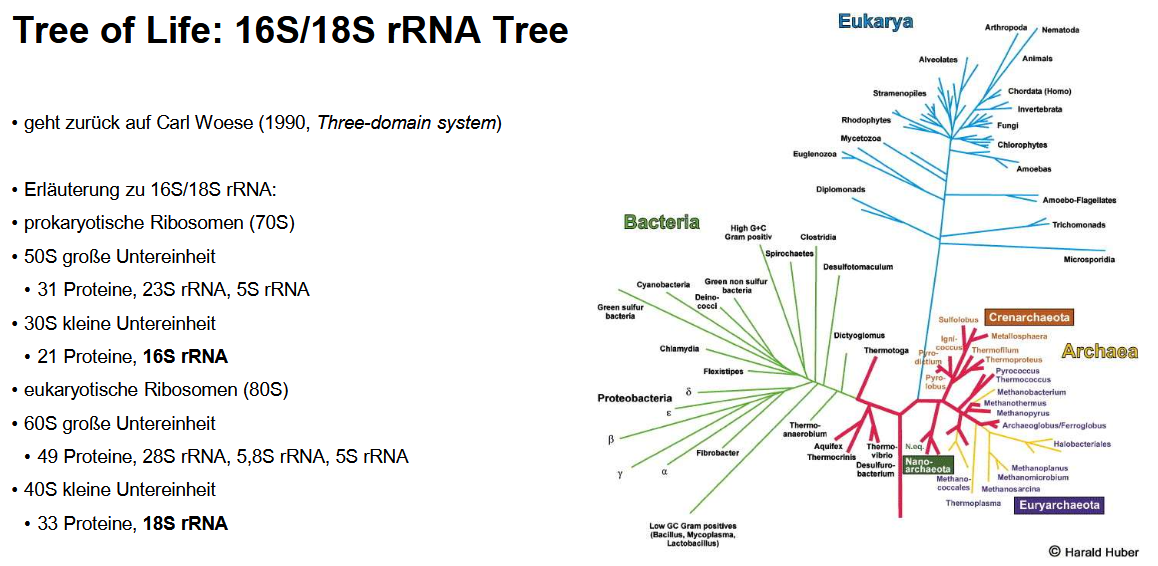
\includegraphics[width=0.8\linewidth]{images/ToF.PNG}
    \caption{Tree of Life}
    \label{fig:treeoflife}
\end{figure}
\paragraph{Die 16S rRNA Phylogenie} ist Phylogenie basierend auf der 16S rRNA der kleinen (30S) Untereinheit des prokaryotischen Ribosoms. Das Gen ist hochkonserviert, denn es unterliegt starkem Selektionsdruck, da die rRNA essentiell für die Translation ist. Es verändert sich also sehr langsam über evolutionäre Zeit. Gleichzeitig enthält es variable Regionen (V1–V9), die artspezifische Unterschiede aufweisen. Diese Kombination aus konservierten und variablen Bereichen macht es ideal als molekulare Uhr. \\
Die Analyse ist oft PCR-basiert, dabei stellen Primer Mismatches und chimäre PCR-Produkte Probleme dar. Außeredm kann horizontaler Gentransfer die Phylogenie verzerren. Mehrere Kopien des Gens pro Zelle können leicht unterschiedlich sein, etc. 
\paragraph{Bei der Genom basierten Phylogenie} \index{Phylogenie} findet eine „Verkettung“ aller gemeinsamer single copy Proteinsequenzen für phylogenetische Analysen statt. 
\begin{itemize}
    \item Zunehmende Anzahl sequenzierter genome von Bakterien und Archeen 
    \item "Verkettung" allen gemeinsamer \textbf{single copy} Proteinsequenzen
\end{itemize}
\paragraph{Der Tree of Life} \index{Tree of life} ist passend für Eukaryonten jedoch für Bakterien und Archaeen kontrovers. Hierbei ist die Kritik vor allem bei Inkonsistenzen bei Genomanalysen. Es wurde herausgefunden, dass Unterschiede Analysen unterschiedliche Ergebnisse geben!\\
Des weiteren gibt es Genfaktoren wie:
\begin{itemize}
    \item horizontaler Gentransfer
    \item Rekombination
    \item Gen Verluste
    \item Gen Neubildungen
\end{itemize}
Insgesamt gilt somit zu sagen, dass es nicht richtig messbar und ein unpassendes Modell für Bakterien und Archeen ist.
\section{Syntenie} \index{Syntenie}
\begin{mechanism}[title=Definition Syntenie]
Als Syntenie werden in
der Genomik Gemeinsamkeiten in der Reihenfolge von Genen oder Gensegmenten auf verschiedenen
chromosomalen Abschnitten beim Vergleich zwischen den Genomen von zwei verschiedenen biologischen Arten
bezeichnet.
\end{mechanism} 